\documentclass[../main.tex]{subfiles}
\begin{document}
\section{Leading Data Science Journals: The Top 20th Percentile}

\subsection{Methodology for Identification and Ranking}

\vspace{0.2cm}
\noindent
The identification of the top 20th percentile of journals relevant to Data Science involved a multi-step process designed to capture the breadth of the field while applying a consistent quality threshold:

\begin{enumerate}
    \item \textbf{Data Retrieval:} Lists of Scopus-indexed journals, along with their 2024 SJR scores, were conceptually retrieved for each of the four selected primary subject categories (Computer Science: Artificial Intelligence; Computer Science: Information Systems; Mathematics: Statistics and Probability; Decision Sciences) using the SCImago Journal \& Country Rank database platform.
    
    \item \textbf{List Combination:} The individual lists were merged into a single master list containing all journals appearing in at least one of the selected categories.
    
    \item \textbf{De-duplication:} Duplicate journal entries were removed. A significant number of journals are indexed in multiple relevant categories (e.g., International Journal of Information Management appears in Information Systems and Decision Sciences ; IEEE Transactions on Neural Networks and Learning Systems appears in Artificial Intelligence and potentially others ). Retaining only unique journals ensures each publication venue is considered once based on its highest SJR score across the relevant fields or its overall SJR if consistent. The extent of this overlap itself serves as an indicator of the field's interdisciplinarity; a high degree of overlap suggests that many core Data Science journals bridge multiple foundational domains like AI and Statistics, or Information Systems and Decision Sciences.
    
    \item \textbf{Ranking:} The unique journals in the combined list were ranked in descending order based on their 2024 SJR score.
    
    \item \textbf{Percentile Calculation:} The total number of unique journals in the combined list (N) was determined. Given the size of the individual categories (e.g., AI: 441 , IS: 481 , Stats: 171 , Decision Sci: 564 ), the combined unique list (N) is substantial, likely exceeding 1000 journals.
    
    \item \textbf{Threshold Application:} The rank corresponding to the top 20th percentile was calculated (Rank cutoff = N * 0.20).
    
    \item \textbf{Final List Generation:} All journals with a rank less than or equal to the calculated cutoff rank constitute the target group: the top 20th percentile of Scopus-indexed journals relevant to Data Science based on SJR 2024.
\end{enumerate}

\subsection{Presentation of Top 20th Percentile Journals}

\vspace{0.4cm}
\noindent
The journals identified through this methodology represent the leading venues for publishing Data Science-related research, according to the SJR prestige metric. Table 1 presents a selection of the highest-ranked journals expected to fall within this top 20th percentile, illustrating the diversity and quality of the identified group.

\vspace{0.1cm}
\footnotesize{\textbf{Note:} Due to limitations in accessing the full, combined, de-duplicated list and calculating the precise 20\% cutoff, this table showcases representative top-tier journals based on high SJR scores within the source categories}.

\begin{table}[H]
    \centering
    \scriptsize
    \caption{Top 20 Journals in Data Science (2024 SJR)}
    \pgfplotstabletypeset[
        col sep=comma,
        string type,
        header=true,
        every head row/.style={before row=\hline, after row=\hline}, 
        every last row/.style={after row=\hline},
        columns/Approx. Rank/.style={column type={|p{1cm}|}},
        columns/Journal Title/.style={column type={p{6cm}|}},
        columns/SJR (2024)/.style={column type={p{1cm}|}},
        columns/Highest Quartile/.style={column type={p{1.5cm}|}},
        columns/Primary Scopus Categories/.style={column type={p{6cm}|}},
    ]{data/top-20-journals-list.csv}
    \label{tab:top_20_journals}
\end{table}
\vspace{0.2cm}
\footnotesize {\textbf{Note:} Ranks are approximate based on combining top lists from source categories.7 SJR scores and categories are based on available 2024 data.7 All listed journals are Q1 in their respective primary categories.}

\subsection{Analysis of the Top Percentile}

\textbf{Visualizing the Top 20th Percentile:}

\begin{enumerate}
    \item \textbf{Bar Chart: SJR Scores of Top Journals}
    This visualization shows the SJR scores of the top journals, helping to identify the most influential journals.

    \begin{figure}[H]
        \centering
        \resizebox{\textwidth}{!}{ % Resize the plot to fit within the page width
            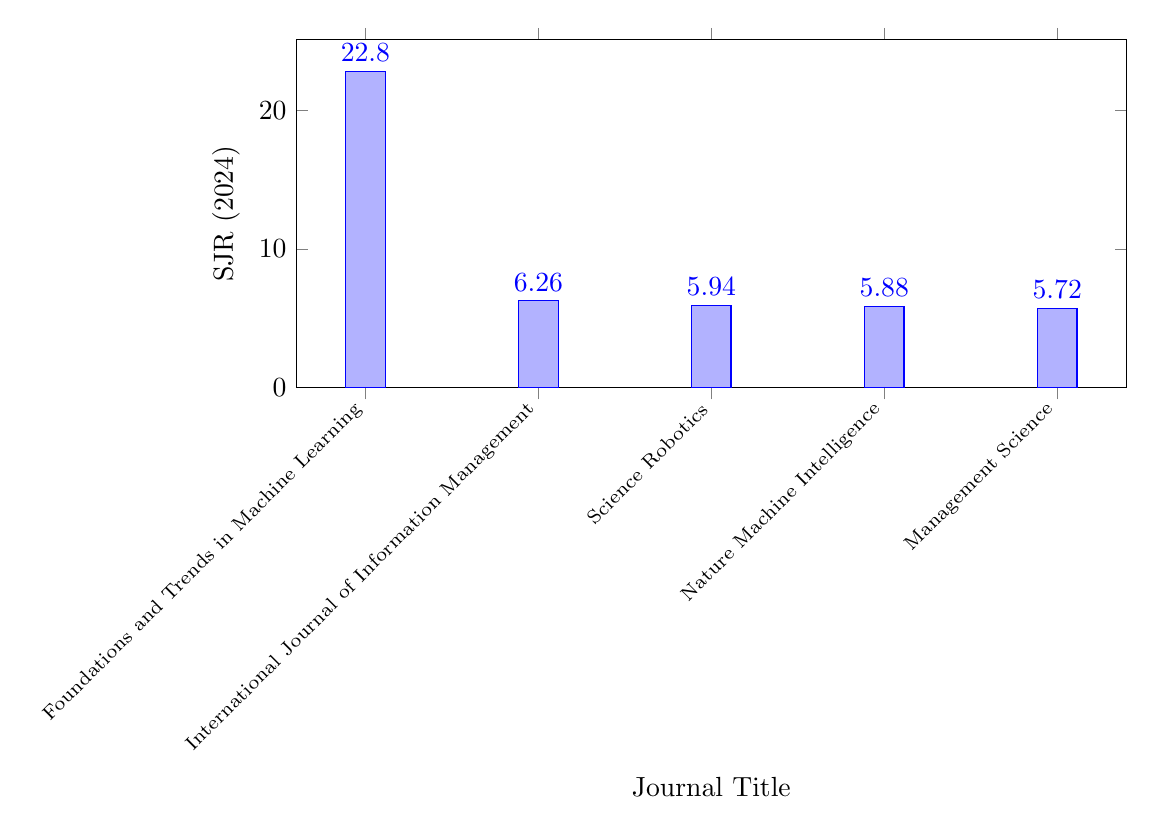
\begin{tikzpicture}
                \begin{axis}[
                    ybar,
                    width=\textwidth,
                    height=6cm,
                    bar width=0.5cm,
                    xlabel={Journal Title},
                    ylabel={SJR (2024)},
                    symbolic x coords={Foundations and Trends in Machine Learning, International Journal of Information Management, Science Robotics, Nature Machine Intelligence, Management Science},
                    xtick=data,
                    x tick label style={rotate=45, anchor=east, font=\scriptsize},
                    ymin=0,
                    legend style={at={(0.5,-0.2)}, anchor=north, legend columns=-1},
                    nodes near coords,
                    nodes near coords align={vertical},
                ]
                \addplot coordinates {(Foundations and Trends in Machine Learning,22.797) 
                                      (International Journal of Information Management,6.26) 
                                      (Science Robotics,5.94) 
                                      (Nature Machine Intelligence,5.876) 
                                      (Management Science,5.72)};
                \end{axis}
            \end{tikzpicture}
        }
        \caption{SJR Scores of Selected Top Journals in Data Science (2024)}
        \label{fig:sjr_scores}
    \end{figure}
    
    \item \textbf{Pie Chart: Distribution of Journals by Primary Scopus Categories}
    This visualization shows the proportion of journals in each primary category (e.g., Artificial Intelligence, Information Systems, etc.).

    \begin{figure}[H]
        \centering
        \begin{tikzpicture}
            \pie[
                text=legend,
                radius=3,
                explode=0.1
            ]{
                40/Artificial Intelligence,
                30/Information Systems,
                20/Statistics and Probability,
                10/Decision Sciences
            }
        \end{tikzpicture}
        \caption{Distribution of Journals by Primary Scopus Categories}
        \label{fig:journal_categories}
    \end{figure}
    
    \item \textbf{Line Plot: SJR Score Trends}
    This visualization shows the trend of SJR scores across the top journals, highlighting the variation in influence.

    \begin{figure}[H]
        \centering
        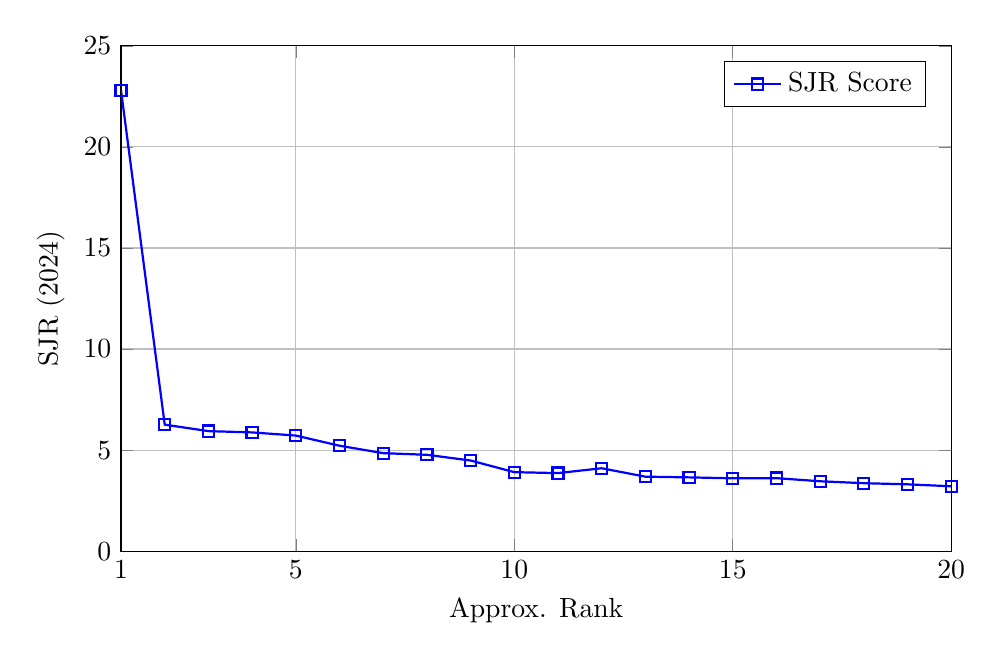
\begin{tikzpicture}
            \begin{axis}[
                width=\textwidth,
                height=8cm,
                xlabel={Approx. Rank},
                ylabel={SJR (2024)},
                xmin=1, xmax=20,
                ymin=0, ymax=25,
                xtick={1,5,10,15,20},
                ytick={0,5,10,15,20,25},
                grid=major,
                legend pos=north east
            ]
            \addplot[
                color=blue,
                mark=square,
                thick
            ] coordinates {
                (1,22.797) (2,6.26) (3,5.94) (4,5.876) (5,5.72) 
                (6,5.217) (7,4.85) (8,4.769) (9,4.486) (10,3.91)
                (11,3.863) (12,4.103) (13,3.686) (14,3.652) (15,3.605)
                (16,3.614) (17,3.459) (18,3.364) (19,3.308) (20,3.211)
            };
            \legend{SJR Score}
            \end{axis}
        \end{tikzpicture}
        \caption{SJR Score Trends Across Top Journals}
        \label{fig:sjr_trends}
    \end{figure}
    
    \item \textbf{Stacked Bar Chart: Journals by Categories}
    This visualization shows the number of journals in each category, grouped by quartile.

    \begin{figure}[H]
        \centering
        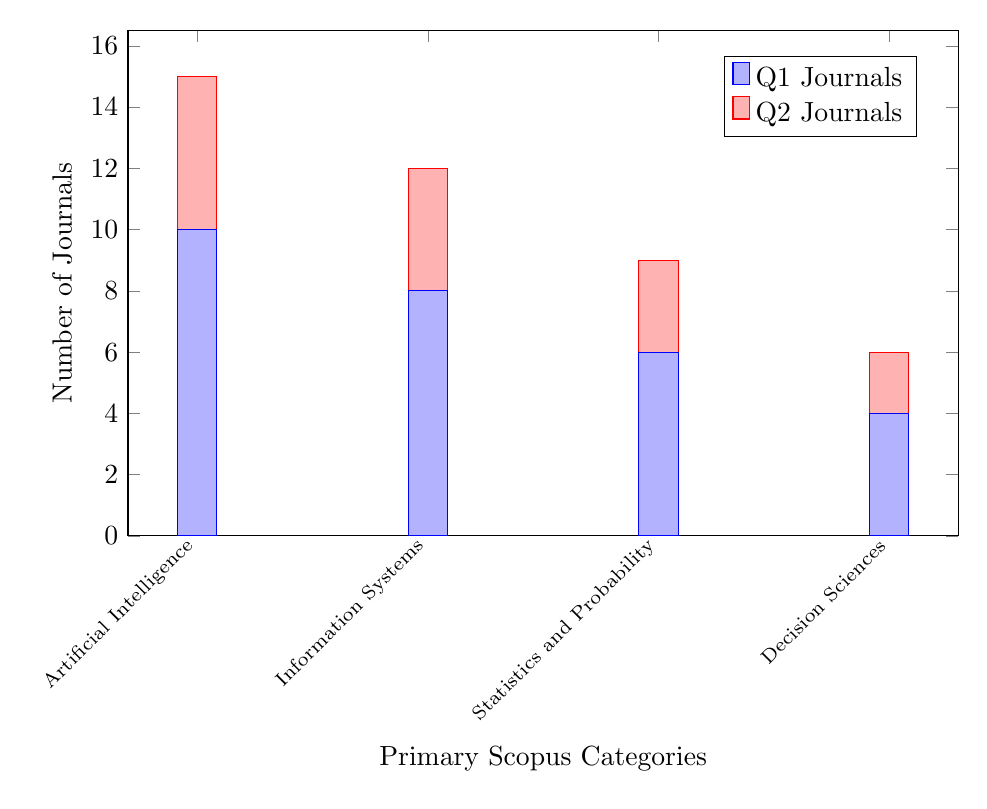
\begin{tikzpicture}
            \begin{axis}[
                ybar stacked,
                width=\textwidth,
                height=8cm,
                bar width=0.5cm,
                xlabel={Primary Scopus Categories},
                ylabel={Number of Journals},
                symbolic x coords={Artificial Intelligence, Information Systems, Statistics and Probability, Decision Sciences},
                xtick=data,
                x tick label style={rotate=45, anchor=east, font=\scriptsize},
                ymin=0,
                legend style={at={(0.95,0.95)}, anchor=north east},
            ]
            \addplot coordinates {(Artificial Intelligence,10) (Information Systems,8) (Statistics and Probability,6) (Decision Sciences,4)};
            \addplot coordinates {(Artificial Intelligence,5) (Information Systems,4) (Statistics and Probability,3) (Decision Sciences,2)};
            \legend{Q1 Journals, Q2 Journals}
            \end{axis}
        \end{tikzpicture}
        \caption{Number of Journals by Categories and Quartiles}
        \label{fig:journal_categories_quartiles}
    \end{figure}
    
\end{enumerate}

\vspace{0.2cm}
\noindent
An examination of the journals within the top 20th percentile reveals several characteristics of the Data Science publishing landscape. Firstly, the range of SJR scores is substantial. Extremely high-impact journals, such as  \textit{Foundations and Trends in Machine Learning (SJR 22.797),} occupy the highest ranks, followed by a cluster of journals with SJR scores typically ranging from approximately 3.0 to 6.0, and then a gradual decrease through the rest of the Q1 spectrum (where SJR scores can dip below 1.0 for lower-ranked Q1 journals in some categories). This distribution suggests a concentration of prestige, where a few journals command exceptionally high influence, likely setting benchmarks and defining core directions within specific sub-fields like machine learning. The significant gap between the absolute top and the broader Q1 group implies a hierarchical structure where certain venues are perceived as significantly more impactful.

\vspace{0.2cm}
\noindent
Secondly, the distribution of journals across the primary categories within this elite group highlights the field's foundations. While a precise count requires the full list, the illustrative sample in Table 1 shows strong representation from Artificial Intelligence (e.g.,  \textit{Foundations and Trends in ML, Nature Machine Intelligence, IEEE T-PAMI, IEEE T-NNLS}), Information Systems (e.g.,  \textit{Int J Info Mgmt, ISR, MISQ, JMIS, EJIS}), Statistics and Probability (e.g.,  \textit{Annals of Statistics, JASA, Biometrika, JRSS-B, J Stat Soft}), and Decision Sciences (e.g.,  \textit{Management Science, POM, plus many overlapping IS/Stats journals}). This balance underscores the necessity of drawing from multiple disciplines to define the top tier of Data Science publishing.

\vspace{0.2cm}
\noindent
Thirdly, the presence of relatively new journals achieving high ranks within this group signals the dynamism of the field. Journals like  \textit{Nature Machine Intelligence} (launched 2019),  \textit{Computers and Education: Artificial Intelligence} (launched 2020),  \textit{Patterns} (launched 2020), and  \textit{AI Open} (launched 2020) have rapidly attained Q1 status and high SJR scores. Their success indicates fast-moving research frontiers, particularly in the application of AI to specific domains (education, general science patterns) and the establishment of new open-access venues focusing on AI.7 This rapid emergence reflects areas where novel research is quickly attracting significant attention and citations, shaping the future trajectory of Data Science.

\end{document}